\chapter{Implementation Specific Details}

The concept of Host Compiled Simulation (HCS) was discussed from a general perspective in Chapter 2. In this work, the technique was implemented to benchmark performance of a target processor based on ARM Cortex A5 Core. In this chapter, the features of the target processor have been discussed. The implementation specific details about the technique have been discussed. 

This discussion will be helpful in identifying the limitations of the approach. It will also lay ground for future contributions to the technique.

\section{Target Processor: Salient Features}

The target processor uses an ARM Cortex A5 core. The salient features are as follows,

\begin{itemize} \itemsep -4pt
\item Single Core Processor
\item In-order Execution Pipeline
\item Dynamic Branch Prediction
\item Separate L1 Cache for Data and Instructions
\item External L2 Cache. Single Cache for Data and Instructions.
\end{itemize}

\section{Instruction Pipeline}
The ARM Cortex A5 Core has an 8 stage pipeline. The stages in the pipeline are shown in Figure \ref{fig:pipelineA5}.

%\vspace*{-30pt}
\begin{figure}[h]
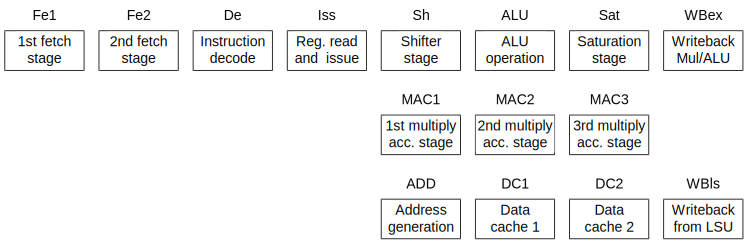
\includegraphics[width=\textwidth]{figures/pipeline.png}
\caption{Pipeline Stages in ARM Cortex A5 Core \cite{CortexA5TRM}}
\label{fig:pipelineA5}
\end{figure}

%TODO: Refine this.
The first 4 stages are common for all instructions. The next stages are specialized for different types of instructions to reduce interlocking. The Shifter, ALU and Saturation stages are used for Arithmetic and Logical Instructions. The multiplication instruction are executed in 3 multiply accumulate stages. For load store instructions, a separate pipeline is implemented. The pipeline stalls when L1 cache miss occurs and data must be fetched from lower levels of cache or main memory. The result is written back to registers in the last stage.

\subsection{Interlocking}
Interlocking can frequently occur in a pipeline due to presence of Data and Control Dependencies among consecutive instructions. An understanding of interlocking behaviour in the Cortex A5 pipeline is important to estimate the number of cycles spent in execution of each basic block. 

As discussed in Section [TODO], the number of cycles spent in execution of each basic block in the pipeline is executed by static analysis. Instructions can have complex dependencies. An accurate estimate is difficult to achieve using static analysis. The ARM Reference Manual \cite{CortexA5TRM} states that for precise timings a cycle-accurate model of the processor must be used. The technique implemented in this project, will give cycle-approximate estimates and could lead to minor inaccuracies.

\vspace*{-10pt}
\paragraph{Operand Forwarding}
To reduce the loss of cycles due interlocking, most modern processors use the technique called Operand Forwarding. Result of an instruction can be forwarded as an input to the next instruction, as soon as it has been evaluated. The Cortex A5 supports Operand Forwarding.

\vspace*{-10pt}
\paragraph{Result Latency}
Result Latency of an instruction is the number of cycles before the result of the instruction is available to be used by the next instruction. Operand Forwarding is taken into account when calculating Result Latency of instructions.

%TODO: Alignment of Example and Text
\begin{Example}
\begin{lstlisting}
LDR R1, [R2]                    ;Result latency three
ADD R3, R3, R1                  ;Register R1 required by ALU
\end{lstlisting}
\end{Example}
\vspace*{-10pt}

For above sequence of instructions, the pipeline will be stalled for 3 cycles.

\vspace*{-10pt}
\paragraph{Early Register}
An Early Register is a register that is needed at the start of Sh, MAC1 or ADD stage (refer to Figure \ref{fig:pipelineA5}) in execution. One more cycle is added to the result latency of the previous instruction producing this register for interlock calculations.

\begin{Example}
\begin{lstlisting}
LDR R1, [R2]                    ;Result latency three
ADD R3, R3, R1    LSL#6         ;plus one, Register R1 is required by Sh
\end{lstlisting}
\end{Example}

In the above example, the value of R1 is needed by the ADD instruction in the Shifter Stage. The pipeline will be stalled for 4 cycles.

\vspace*{-10pt}
\paragraph{Late Register}
A Late Register is not required until the start of the ALU, MAC1 or DC1 stage for the second execution. One cycle is subtracted from the result latency of the previous instruction producing this result for interlock calculations.

\begin{Example}[h]
\begin{lstlisting}
LDR R1, [R2]                    ;Result latency three
ADD R3, R3, R1, R4 LSL#5        ;minus one, Register R1 is a Late Reg
\end{lstlisting}
\end{Example}

In the above example, the pipeline is stalled for only 2 cycles. While the LDR instruction is being executed, the value in R4 is being shifted. After waiting for 2 more cycles, the value of R1 is made available, and execution can proceed.

The binary instructions in each basic block are parsed sequentially. For each instruction, the early and late registers, and corresponding dependencies are identified. Penalties are appropriately added for the pipeline stalls. The results corroborate that the approach is fairly accurate. The accuracy can be further improved by creating a cycle accurate model of the processor pipeline, and simulating the instructions on this model. This will significantly increase the complexity of the approach and the time needed in instrumentation.

\subsection{Branch Prediction Unit}
The specific implementation of the Branch Prediction Algorithm used in the ARM Cortex A5 has not been disclosed in the Reference Manual. However, it is based on the algorithm described in Section [TODO]. The Cortex A5 uses a 256 table Branch History Table. The simulator models the Branch Prediction Unit, to take into account the effect on the execution time. Results show an average of +20\% error in estimation of the number of branches that were mispredicted.

\section{Memory System}
\label{sec:c3CacheHierarchy}
The Cortex A5 supports separate L1 Caches for Data and Instruction. On the target processor, an external L2 Cache has been used. Table \ref{tbl:cacheSize} shows the parameters for the caches.

%\vspace*{10pt}
\begin{table}[h]
\centering
%\begin{tabularx}{360pt}{>{\centering\arraybackslash}X>{\centering\arraybackslash}X>{\centering\arraybackslash}X>{\centering\arraybackslash}X}
\begin{tabular}{cccc}
    \toprule
        &  Size   & N-way   & Cache Line Size \\
    \hline
    L1 D Cache  & 32 KB & 4 & 32 B \\
    L1 I Cache  & 32 KB & 2 & 32 B \\
    L2 Cache    & 512 KB & 16 & 32 B \\
    \bottomrule
\end{tabular}
%\end{tabularx}
\caption{Size of Caches}
\label{tbl:cacheSize}
\end{table}

To estimate the time spent in accessing memory, a Cache Simulator has been developed. In order to keep reduce the implementation complexity, and increase the execution speed a Cycle-Approximate Cache Simulation is used. This could result in inaccuracies. For precise estimates, a cycle accurate Cache Simulator can be implemented. 

Results show that the error in estimation of number of cache misses is negligible. However, inaccurate timing estimates have contributed to the error in estimate cycle counts. 

The features of the Cortex A5 memory system have been described. Details of how these features were implemented in the Cache Simulator have been discussed. The following section also highlights the possible source of inaccuracy in estimation.

\subsection{Replacement Policies}
The L1 Caches use a Pseudo Random Replacement Policy, while the L2 Cache used Round Robin Replacement Policy. The Cortex A5 uses and Exclusive Cache Mode. In this mode, a given address is cached in either L1 Cache or in L2 Cache, but not in both. 

This has the effect of increasing the usable space and efficiency. The data is loaded from memory into L1 Cache. On eviction from L1, the data is stored in the L2 Cache. This feature has been simulated in the Cache Simulator.

\subsection{Data Prefetching}
Cortex A5 also supports prefetching of data. The addresses fetched from memory are analysed and spatial locality of accesses is identified. Data which is highly probable of being used by the application is prefetched in the L1 Cache.

This feature has a significant impact on performance. The specific implementation of the Data Prefetching Unit has not been disclosed. The simple technique implemented in Cache Simulator to imitate the Branch Prediction Unit, does not show accurate results. Average error of 60\% was observed. 

\subsection{Read-Allocate Mode}
The L1 and L2 Caches used on the target processor are Write-Back Caches. Data is written to the L1 Cache before being written to the main memory. When a store operation is executed, the address is looked up in the L1 Cache. If the address is not found, a write-miss occurs and data must be fetched from L2 or the main memory. The updated data is stored in the L1 Cache. 

However, functions like \emph{memset} are used to write to a large area of memory, with the same value. Allocating this memory in the L1 Cache pollute the cache. For such cases, the processor switches to a Read-Allocate Mode. In this mode, memory is allocated in L1 Cache only for read accesses. Writes are done to the L2 Cache instead.

Implementing this feature in the Cache Simulator will adversely impact the speed of execution of the simulation. This feature has not been implemented in the Cache Simulator, and may be the cause for some inaccuracy in results. The Cache simulator can be extended to support this feature.

\subsection{Store Buffers}
To speed up memory write operations, store buffers are used in the Cortex A5. When dirty data is evicted from L1 Cache, it is written to the store buffers of the L2 Cache. This data will asynchronously be written to the L2 Cache later. The Cortex A5 uses a [TODO] store buffers.

Simulating Store Buffers in a cycle accurate fashion is difficult. In this project, it has been assumed that evict operations from L1 cache to L2 cache will work without any latency. However, this results in inaccuracies in the test cases that write a large amount of data to the memory. The pressure on the store buffers can not be taken into account. 

